\documentclass[english,version-2020-11]{uzl-thesis}


\UzLThesisSetup{
  Masterarbeit,
  Logo-Dateiname        = {uzl-thesis-logo-itcs.pdf},
  Verfasst              = {am}{Institut für Theoretische Informatik},
  Titel auf Deutsch     = {Über elementare Eigenschaften einer mehrdimensionalen Verallgemeinerung des euklidischen Algorithmus},
  Titel auf Englisch    = {On Elementary Properties of a Multi-Dimensional Generalization of the Euclidean Algorithm},
  Autor                 = {Daniel Knaack},
  Betreuerin            = {Prof. Dr. Kim-Manuel Klein},
  Studiengang           = {Informatik},
  Datum                 = {18. Juni 2024},
  Abstract              = {TODO},
  Zusammenfassung       = {TODO},
  Numerische Bibliographie,
}

\UzLStyle{alegrya modern design}

\begin{document}

\chapter{Introduction}

\chapter{Preliminaries}

\section{Generalized Euclidean Algorithm}

\begin{Pseudocode}
while $x$ is not integral do
  solve $Bx = c$
  find $x_l$ which is not integral
  swap $B_l$ and $c$
  ...
end
\end{Pseudocode}

\chapter{Bounds on the Determinant}

\[
  K_n(x_1, \dots, x_n) =
  \begin{cases}
    1, & \text{ if } n = 0, \\
    x_1, & \text{ if } n = 1, \\
    x_1 K_{n-1}(x_2, \dots, x_n) + K_{n-2}(x_3, \dots, x_n), & \text{ otherwise.}
  \end{cases}
\]

The Euclidean algorithm takes exactly $n$ steps if $a$ has a minimal continued
fraction with $n$ terms $[a_0; a_1, a_2, \dots, a_n]$. For the generalized
algorithm, it takes as long as the length of the longest continued fraction.

\begin{theorem}
  The determinant $\det(B)$ decreases by a factor of at least $\phi^{-2d}$ over
  $2d$ iterations.
\end{theorem}

\begin{proof}
  Assume there is some solution vector $x$ with $x_i > 1/\phi$ for all $i$
  such that the decrease is slower than $1/\phi$ over $d+1$ iterations.
  Because $1/x_i < \phi$ and $\phi - 1 = 1/\phi$,
  the next value $1/x_i - 1$ must be smaller than $1/\phi$,
  Therefore, choosing
\end{proof}

\section{What Makes a Bad Solution?}

In one dimension, a solution is bad when the value $x_1$ is close to $1$.
However, in the next iteration $x_1$ would be close to $0$ and therefore
would lead to a greater decrease in the determinant.
An initial guess would be that the solution lies exactly between $0$ and $1$ at $1/2$.
However, this solution is also good as after just one step we have achieved integrality.

The solution is to choose a value $x_1$ such that its value in the first
iteration is the same as its value in the second iteration.
This means we are trying to solve the following equation:
\[
  x_1 = 1/x_1 - 1.
\]
This gives us the polynomial $x^2 + x - 1$ where the root is the inverse of the
golden ratio.

% TODO: Explore other strategies. Can we generalize this to every possible strategy?
In just two dimensions, we already have an additional degree of freedom.
Since the solution $x$ consists of two values, we can choose which index we pivot with.
We will choose the value with the smallest fractional value as this decreases
the determinant the fastest.
We assume w.l.o.g. that our values are sorted in increasing order.
This means we pivot with $x_1$ first.

% TODO: What about just choosing the golden ratio for every x_i?
% TODO: Are odd dimensions easier since the decrease is not worse? We could
% choose two values to be the same, since the ratio for odd dimensions is
% smaller than the previous dimension
Just like in one dimension we want to choose $x_1$ carefully such that the
determinant decreases the same amount in every iteration.
A simple solution would be to fill both values with the golden ratio.
In this case, it does not matter which index we choose as each one decreases
the determinant the same amount.
However, in two dimensions we can make this decrease slightly worse
by choosing different values for $x_1$ and $x_2$ such that we swap the pivot
in each iteration.

Assuming the value for $x_1$ is already chosen where would $x_2$ be placed?
Ideally, it would be close to the right side of $x_1$, because then the new
value $-x_2 / x_1$ would be close to $-1$ and the fractional value would be
close to $1$.
Since the decrease must stay the same in each iteration, this gives us the
following two equations:
\begin{align*}
  x_1 = 2 - x_2 / x_1 \\
  x_2 = 1 / x_1 - 1,\\
\end{align*}
which leads to the following polynomial:
\begin{align*}
  x_1^3 - 2x_1^2 - x_1 + 1 = 0
\end{align*}

Let $\phi_2$ be the root of this polynomial.
If we choose $x_1 = \phi_2$ and $x_2 = 2\phi_2 - \phi_2^2$,
then the values in the second iteration are
\[\begin{aligned}
  x_1' & = 1 / x_1 - 1   &  & = 1 / \phi_2 - 1                    &  & = 2\phi_2 + \phi_2^2 &  & = x_2, \\
  x_2' & = 2 - x_2 / x_1 &  & = 2 - (2\phi_2 + \phi_2^2) / \phi_2 &  & = \phi_2             &  & = x_1
\end{aligned}\]

We can extend this to $d$ dimensions using the following equations:
\begin{align*}
  x_1 = 2 - x_2 / x_1 \\
  x_2 = 2 - x_3 / x_1 \\
  x_3 = 2 - x_4 / x_1 \\
  \vdots \\
  x_{d-1} = 2 - x_d / x_1 \\
  x_d = 1 / x_d - 1 \\
\end{align*}

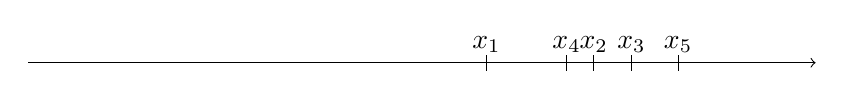
\begin{tikzpicture}[scale=10]
  \draw (0.5820216424559055, -0.01) -- node[above] {$x_1$} (0.5820216424559055, 0.01);
  \draw (0.7181491667223714, -0.01) -- node[above] {$x_2$} (0.7181491667223714, 0.01);
  \draw (0.7661126076135922, -0.01) -- node[above] {$x_3$} (0.7661126076135922, 0.01);
  \draw (0.6837042616132034, -0.01) -- node[above] {$x_4$} (0.6837042616132034, 0.01);
  \draw (0.8252940926247403, -0.01) -- node[above] {$x_5$} (0.8252940926247403, 0.01);
  \draw[->] (0, 0) -- (1, 0);
\end{tikzpicture}

\section{Fibonacci Numbers}

\begin{itemize}
  \item Fibonacci numbers are just linear recurrences with constant coefficients $c_0 = 1, c_1 = 1$.
  \item Linear recurrence with coefficients $c_0, c_1, \dots, c_d$: $a_{n+d+1} = \sum_{i=0}^d c_i a_{n+i}$.
  \item The characteristic polynomial of the Fibonacci sequence is the polynomial of the golden ratio.
  \item For even dimensions: $c_0 = -1, c_1 = 1, c_2 = 2, c_3 = -2, \dots, c_{2d-1} = -2, c_{2d} = 2$.
  \item For odd dimensions:  $c_0 = 1, c_1 = -1, c_2 = -2, c_3 = 2, \dots, c_{2d} = -2, c_{2d+1} = 2$.
  \item The ratio $\phi_d$ for the characteristic polynomials approaches $1/\sqrt{3}$ as $d \to \infty$.
  \item Folding an A4 paper?
\end{itemize}

\chapter{$d$-bonacci Number}

\section{Multi-Dimensional Golden Ratio}

\begin{definition}[$d$-dimensional Golden Ratio]
  The $d$-dimensional golden ratio is the only positive real root $\phi_d$ of the polynomial:
  \[
    x^{d+1} + x^d + \dots + x^2 + x = 1.
  \]
\end{definition}

All sums of the form $\sum_{k=1}^i \phi_d^k$ with $i \le d$ must be strictly less than one.

Dividing by $x$ on each side gives us the following equation:
\[
  x^d + x^{d-1} + \dots + x + 1 = 1/x.
\]

% TODO: Explain why we can subtract one from each.
We choose $x_i = \sum_{k = 1}^i \phi_d^k$.
The values are ordered such that $x_1$ is the smallest value.
Therefore we begin pivoting with $x_1$.
After the update, the new value for $x_1$ is
\[
  x_1' = 1/\phi_d - 1 = \phi_d^d + \phi_d^{d-1} + \dots + \phi_d = x_d.
\]
The other values of the new solution are
\[
  x_i' = x_i / x_1 - 1 = \sum_{k = 1}^i \phi_d^k / \phi_d - 1 = \sum_{k=1}^{i-1} \phi_d^k.
\]
Hence, we rotate the values forwards, so that $x_i' = x_{i-1}$ and $x_1' = x_d$.
In the next iteration we would choose $x_2$ as our pivot since it is the smallest value.

\section{Higher-Order Fibonacci Numbers}

\begin{definition}
  The \emph{$d$-bonacci numbers} are defined as follows:
  \begin{enumerate}
    \item $F_d(0) = F_d(1) = \dots = F_d(d) = 0$.
    \item $F_d(n) = \sum_{i = 1}^{d+1} F_d(n - i)$ for $n > d$.
  \end{enumerate}
\end{definition}

Using the $d$-bonacci numbers, we can approximate the golden ratio $\phi_d$
by computing the ratio between consecutive terms $F_d(n - 1) / F_d(n)$.
Furthermore, we can approximate powers of the golden ratio by increasing the distance between the terms.
For example, we can approximate $\phi_d^2$ by the term $F_d(n - 2) / F_d(n)$.

In order to prove that the ratios approximate $\phi_d$,
we first prove the convergence criteria for this sequence, i.e.
the sequence is bounded and is monotonically increasing.

\begin{lemma}
  The ratio $F_d(n - i) / F_d(n)$ is bounded between $0$ and $1$.
\end{lemma}

\begin{proof}

\end{proof}

\begin{lemma}
  The ratios are monotonically increasing with increasing $n$.
\end{lemma}

\begin{proof}

\end{proof}

\begin{theorem}
  $\lim_{n \to \infty} F_d(n - k) / F_d(n) = \phi_d^i$ for $i \ge 1$.
\end{theorem}

\begin{proof}
  We begin with $k = 1$.
  By the previous lemmas, we can assume that the ratio approaches some limit $L$:
  \begin{align*}
    \lim_{n \to \infty} \frac{F_d(n - 1)}{F_d(n)} = L.
  \end{align*}
  From the definition of the $d$-bonacci numbers, we can rewrite $F_d(n - 1)$ as follows:
  \begin{align*}
    F_d(n) & = F_d(n - 1) + \dots + F_d(n - d - 1) \\
    \Leftrightarrow F_d(n - 1) & = F_d(n) - F_d(n - 2) - \dots - F_d(n - d - 1)
  \end{align*}
  This gives us the following equation for the limit $L$:
  \begin{align*}
    L = \lim_{n \to \infty} \frac{F_d(n - 1)}{F_d(n)}
      = \lim_{n \to \infty} 1 - \frac{\sum_{i=2}^{d+1} F_d(n - i)}{F_d(n)}
      = 1 - \sum_{i=2}^{d+1} \lim_{n \to \infty} \frac{F_d(n - i)}{F_d(n)}
  \end{align*}
  Each term in the sum can be rewritten as the ratio of two consecutive $d$-bonacci numbers:
  \begin{align}
    \label{eq:power}
    \lim_{n\to\infty} \frac{F_d(n - i)}{F_d(n)} = \lim_{n\to\infty}\frac{F_d(n - i)}{F_d(n - i + 1)} \cdot \ldots \cdot \frac{F_d(n - 1)}{F_d(n)} = L^i.
  \end{align}
  Therefore, as $n$ approaches infinity each term in the sum approaches a power of $L$:
  \begin{align*}
    L = \lim_{n \to \infty} \frac{F_d(n - 1)}{F_d(n)}
      = 1 - \sum_{i=2}^{d+1} \lim_{n \to \infty} \frac{F_d(n - i)}{F_d(n)}
      = 1 - L^2 - L^3 - \dots - L^{d+1}
  \end{align*}
  Per definition, the solution to this equation is exactly $\phi_d$.
  The limit for $k > 1$ follows directly from Equation~\ref{eq:power}.
\end{proof}

Using this theorem, we can swap out the power-sum of $\phi_d$ in the solution
vector from the previous section with sums of consecutive $d$-bonacci terms.
We set $x_i = \sum_{k=1}^i (-1)^k F_d(n - k) / F_d(n)$ and pivot with $x_1$.
The new value for $x_1$ is
\[
  x_1'
  = \{1/x_1\}
  = \frac{F_d(n)}{F_d(n - 1)} - 1
  = \sum_{k=1}^{d+1} (-1)^{k + 1} \frac{F_d(n - k)}{F_d(n - 1)} - 1
  = \sum_{k=1}^d (-1)^k \frac{F_d(n - 1 - k)}{F_d(n - 1)}
\]
and the new values for $x_i$ are
\[
  x_i'
  = -x_i / x_1
  = -\sum_{k=1}^i (-1)^k \frac{F_d(n - i)}{F_d(n)} \frac{F_d(n)}{F_d(n - 1)}
  = \sum_{k=1}^{i-1} (-1)^k \frac{F_d(n - 1 - i)}{F_d(n - 1)}.
\]

% TODO: How would we choose the matrix? Can

\chapter{Bounds (old)}

\begin{itemize}
  \item We choose the smallest index in each iteration since this gives us the
    largest change in the determinant.
\end{itemize}

Assumption:
\[
  x_1 = \frac{x_2}{x_1} - 1 = \dots = \frac{x_{d}}{x_{d-1}} - 1 = \frac{1}{x_d} - 1,
\]
which leads to the following polynomials:
\begin{align}
  \label{eq:solution}
  x_d^{d+1} + x_d - 1 = 0 \quad \text{ and } \quad x_i = x_d^{d - i + 1}.
\end{align}

In one dimension, the root of the polynomial $\phi_1$ is the \emph{inverse of the golden ratio}.
In two dimension, the root of the polynomial $\phi_2$ is the \emph{inverse of the supergolden ratio}.
Hence, we have to substitute $x$ with the inverse of $y$ to get the actual golden ratio:

\begin{align*}
  (1/y)^{d+1} + 1/y - 1       & = 0 \quad \text{(Expand second term with $y^d$)} \\
  1/y^{d+1} + y^d/y^{d+1} - 1 & = 0 \quad \text{(Multiply with $y^d$)}           \\
  1 + y^d - y^{d+1}           & = 0 \quad \text{(Multiply with $-1$)}            \\
  y^{d+1} - y^d - 1           & = 0                                              \\
\end{align*}

Let $\phi_d$ be the root of this polynomial.
For $d = 1$, the root $\phi_1$ is the \emph{golden ratio}.
For $d = 2$, the root $\phi_2$ is the \emph{supergolden ratio}.

The golden ratio can be approximated using the Fibonacci sequence,
the super golden ratio can be approximated using Narayana's cow sequence:

\begin{align*}
  F(0) = F(1) = 1,        & \quad F(n) = F(n - 1) + F(n - 2), n \ge 2 \\
  N(0) = N(1) = N(2) = 1, & \quad N(n) = N(n - 1) + N(n - 3), n \ge 3
\end{align*}

From the Narayana sequence, we can naturally generalize the sequence to higher dimensions:

\[
  F_d(0) = F_d(1) = \dots = F_d(d) = 1, \quad F_k(n) = F_d(n - 1) + F_d(n - d - 1).
\]

\begin{table}[t]
  \caption{The first 18 Fibonacci numbers of orders one to five.}
  \begin{tabular}{c|cccccccccccccccccccc}
    $n$     & 0 & 1 & 2 & 3 & 4 & 5 & 6 & 7  & 8  & 9  & 10 & 11 & 12  & 13  & 14  & 15  & 16  & 17   \\ %& 18   & 19   \\
    \hline
    $F_1(n)$ & 0 & 1 & 1 & 2 & 3 & 5 & 8 & 13 & 21 & 34 & 55 & 89 & 144 & 233 & 377 & 610 & 987 & 1597 \\ %& 2584 & 4181 \\
    $F_2(n)$ & 0 & 1 & 1 & 1 & 2 & 3 & 4 & 6  & 9  & 13 & 19 & 28 & 41  & 60  & 88  & 129 & 189 & 277  \\ %& 406  & 595  \\
    $F_3(n)$ & 0 & 1 & 1 & 1 & 1 & 2 & 3 & 4  & 5  & 7  & 10 & 14 & 19  & 26  & 36  & 50  & 69  & 95   \\ %& 131  & 181  \\
    $F_4(n)$ & 0 & 1 & 1 & 1 & 1 & 1 & 2 & 3  & 4  & 5  & 6  & 8  & 11  & 15  & 20  & 26  & 34  & 45   \\ %& 60   & 80   \\
    $F_5(n)$ & 0 & 1 & 1 & 1 & 1 & 1 & 1 & 2  & 3  & 4  & 5  & 6  & 7   & 9   & 12  & 16  & 21  & 27   \\ %& 34   & 43   \\
  \end{tabular}
\end{table}

Any two consecutive terms can be used to approximate the corresponding ratio, i.e. $\lim_{n \to \infty} F_d(n) / F_d(n + 1) = \phi_d$.

Going back to the Euclidean algorithm,
an example matrix which leads to the solution given by Equation~\ref{eq:solution} is:
\begin{align*}
  \left(\begin{array}{ccccc|c}
    a^d    & 0       & \cdots & 0      & 0      & b^d     \\
    0      & a^{d-1} & \cdots & 0      & 0      & b^{d-1} \\
    \vdots & \vdots  & \ddots & \vdots & \vdots & \vdots  \\
    0      & 0       & \cdots & a^2    & 0      & b^2     \\
    0      & 0       & \cdots & 0      & a      & b       \\
  \end{array}\right),
\end{align*}
where $a = F_d(n)$ and $b = F_d(n + 1)$.

\section{Multi-Dimensional Golden Ratio and Higher-Order Fibonacci Numbers}

\begin{definition}
  The $d$-dimensional golden ratio $\phi_d$ is the real positive root of $x^{d+1} - x^d - 1$.
\end{definition}

\begin{definition}
  The $d$-th order Fibonacci numbers are defined as follows:
  \begin{itemize}
    \item $F_d(0) = F_d(1) = \dots = F_d(d-1) = 1$,
    \item $F_d(n) = F_d(n-1) + F_d(n-d-1)$ for $n \ge d$.
  \end{itemize}
\end{definition}

\begin{lemma}
  The sequence $R_d(n+d)$ can be reformulated as follows:
  \begin{align*}
    R_d(n+d)
    & = 1 + \frac{1}{R_d(n+d-1) R_d(n+d-2) \dots R_d(n)}
  \end{align*}
\end{lemma}

\begin{proof}
  \begin{align*}
    R_d(n+d)
    & = \frac{F_d(n+d+1)}{F_d(n+d)}
    = \frac{F_d(n+d) + F_d(n)}{F_d(n+d)}
    = 1 + \frac{F_d(n)}{F_d(n+d)} \\
    & = 1 + \frac{F_d(n)}{R_d(n+d-1) F_d(n+d-1)}
    = 1 + \frac{F_d(n)}{R_d(n+d-1) R_d(n+d-2) F_d(n+d-2)} \\
    & \mathrel{\vdots} \\
    & = 1 + \frac{F_d(n)}{R_d(n+d-1) R_d(n+d-2) \dots R_d(n) F_d(n)} \\
    & = 1 + \frac{1}{R_d(n+d-1) R_d(n+d-2) \dots R_d(n)}
    \qedhere
  \end{align*}
\end{proof}

\begin{lemma}
  The sequence $R_d(n) = F_d(n+1) / F_d(n)$ is bounded between $1$ and $2$.
\end{lemma}

\begin{proof}
  For all $n < d - 1$ this is obviously the case.
  Per induction, assume that $R_d(n), R_d(n+1), \dots, R_d(n+d-1)$ are bounded.
  From the previous lemma, we know
  \begin{align*}
    R_d(n+d)
    & = 1 + \frac{1}{R_d(n+d-1) R_d(n+d-2) \dots R_d(n)}
  \end{align*}
  By the induction hypothesis, each ratio is bounded between $1$ and $2$.
  Therefore, $R_d(n+d)$ is equally bounded between $1$ and $2$.
\end{proof}

\begin{lemma}
  The sequence $R_d(n)$ is monotonically increasing.
\end{lemma}

\begin{proof}

\end{proof}

\begin{theorem}
  The sequence $F_d(n + k) / F_d(n)$ for $k \ge 1$ converges to $\phi_d^k$.
\end{theorem}

\begin{proof}
  From the previous two lemmas, we know that the sequence converges.
  Therefore, there exists some $L$ such that
  \[
    \lim_{n \to \infty} R_d(n) = \lim_{n \to \infty} 1 + \frac{1}{R_d(n-1) R_d(n-2) \dots R_d(n-d)} = L.
  \]
  As $n$ approaches infinity, all ratios approach some limit $L$.
  Hence, $L = 1 + 1/L^d$ or equivalently $L^{d+1} - L^d - 1 = 0$,
  which fits the definition of the golden ratio $\phi_d$.
\end{proof}

From the previous theorem, we can construct a matrix $A$ and vector $b$ such that the solution
still approximates the powers of $\phi_d$ but with significantly smaller terms:

\begin{align*}
  A = \begin{pmatrix}
    F_d(n + d) \\
    & F_d(n + d - 1) \\
    && \ddots \\
    &&& F_d(n + 2) \\
    &&&& F_d(n + 1) \\
  \end{pmatrix},
  b =
  \begin{pmatrix}
    F_d(n) \\
    F_d(n) \\
    \vdots \\
    F_d(n) \\
    F_d(n) \\
  \end{pmatrix}
\end{align*}

The most fractional index in the solution is $x_d$ since it approximates $1/\phi_d$,
while the other terms approximate powers of $1/\phi_d$ and are therefore smaller.
Pivoting once with $d$, reduces the power of each term $x_i$ with $i \ne d$.
However, at the same time it increases the power of $x_d$, because now $x_d$ has the following value:
\[
  x_d' = 1/x_d - 1 = \frac{F_d(n+1)}{F_d(n)} - 1 = \frac{F_d(n) + F_d(n - d)}{F_d(n)} - 1 = \frac{F_d(n - d)}{F_d(n)}.
\]
Again, from the previous theorem it follows that the next solution $x_d'$ would approach $\phi_d^d$ as $n$ goes to infinity.
For the other terms, we reduce each by one power:
\begin{align*}
  x_i'
  & = x_i/x_d - 1 \\
  & = \frac{F_d(n)}{F_d(n + d + 1 - i)} \cdot \frac{F_d(n + 1)}{F_d(n)} - 1 \\
  & = \frac{F_d(n + d - i)}{F_d(n + d + 1 - i)} \cdot \dots \cdot \frac{F_d(n)}{F_d(n + 1)} \cdot \frac{F_d(n + 1)}{F_d(n)} - 1 \\
  & = \frac{F_d(n + d - i)}{F_d(n + d + 1 - i)} \cdot \dots \cdot \frac{F_d(n+1)}{F_d(n + 2)} \frac{F_d(n)}{F_d(n + 1)} \cdot \frac{F_d(n + 1)}{F_d(n)} - 1 \\
  & = \frac{F_d(n + d - i)}{F_d(n + d + 1 - i)} \cdot \dots \cdot \frac{F_d(n+2)}{F_d(n + 1)} - 1 \\
  & = \frac{F_d(n + d - i)}{F_d(n + 1)} - 1 \\
\end{align*}

\section{Sums of Higher-Order Fibonacci Numbers}

\begin{lemma}
  \[\sum_{i = 0}^n F_d(i) = F_d(n + 1 + d) - 1.\]
\end{lemma}

\begin{proof}
  Let $n = 0$, then $F_d(d + 1) = F_d(d) + F_d(0) - 1 = 1 + F_d(0) - 1 = F_d(0)$.
  Per induction, assume $\sum_{i=0}^n F_d(i) = F_d(n + 1 + d) - 1$. For $n + 1$, it follows:
  \begin{align*}
    \sum_{i = 0}^{n+1} F_d(i)
    & = F_d(n + 1) + \sum_{i = 0}^n F_d(i) \\
    & = F_d(n + 1) + F_d(n + d) - 1 \\
    & = F_d(n + 1) + F_d(n + 1 + d) - 1 \\
    & = F_d(n + 2 + d) - 1. \qedhere
  \end{align*}
\end{proof}

\begin{lemma}
  \[\sum_{i = k}^n F_d(i) = F_d(n + 1 + d) - F_d(k + 1 + d).\]
\end{lemma}

\begin{proof}
  \begin{align*}
    \sum_{i = k}^n F_d(i)
    & = \sum_{i = 0}^n F_d(i) - \sum_{i = 0}^{k-1} F_d(i) \\
    & = F_d(n + 1 + d) - 1 - F_d(k + d) + 1 \\
    & = F_d(n + 1 + d) - F_d(k + d). \qedhere
  \end{align*}
\end{proof}

\begin{corollary}
  $\sum_{i=k}^n F_d(i) = F_d(n + 1 + d) - F_d(k + 1 + d)$.
\end{corollary}

\section{Generator Matrix for Higher-Order Fibonacci Numbers}

\begin{lemma}[Honsberger's Identity]
  \[
    F_d(n + m) = F_d(m - d) F_d(n) + F_d(m) F_d(n + d).
  \]
\end{lemma}

\begin{definition}[Generator Matrix]
  \[
    G_d := \begin{pmatrix}
      \begin{matrix}
        1 & 0 & \dots & 0
      \end{matrix} & 1 \\
      I_d &
      \begin{matrix}
        0 \\
        \vdots \\
        0 \\
        0 \\
      \end{matrix} \\
    \end{pmatrix} \in \mathbb{N}^{(d+1) \times (d+1)}
  \]
\end{definition}

\begin{itemize}
  \item How could we compute a diagonalization of this matrix?
  \item What is the value of $G_d^n$?
\end{itemize}

\begin{lemma}
  $\det(G_d) = (-1)^d$.
\end{lemma}

\begin{proof}
  We calculate the determinant using Laplace expansion in the first row.
  Taking the first entry $(G_d)_{1,1}$ and removing the first row and column produces
  a lower-triangle matrix with only zeros on its diagonal.
  The determinant for this submatrix is therefore zero.
  For the last entry $(G_d)_{1,d+1}$, we get the identity matrix.
  Hence, the determinant for the matrix is $(-1)^{d+2} = (-1)^d$.
\end{proof}

\begin{lemma}
  The only real positive eigenvalue of $G_d$ is $\phi_d$.
\end{lemma}

\begin{proof}
  We find a $\lambda$ such that $\det(G_d - \lambda I_d) = 0$ using Laplace expansion in the first row.
  Again, only two candidates are of interest: The first column and last column.
  Removing the first column and first row, we get a lower triangle matrix with a diagonal of $-\lambda$.
  Removing the last column and first row, we get an upper triangle matrix with a diagonal of $1$.
  Therefore, the determinant is:
  \[
    \det(G_d - \lambda I_d) = (1 - \lambda^d) (-\lambda^d) + (-1)^d = 0.
  \]
  Multiplying by $(-1)^d$ gives us the polynomial for the golden ratio.
\end{proof}

\begin{lemma}
  The eigenvector of $G_d$ is $v = (\phi_d^d, \phi_d^{d-1}, \dots, \phi_d^1, \phi_d^0)^\top$.
\end{lemma}

\begin{proof}
  The eigenvector of $G_d$ must satisfy $(G_d - \phi_d I_d) v = 0$.
  The first equation in this linear system is $(1 - \phi_d) v_1 + v_d = 0$.
  The $(i+1)$-th equation gives us $v_i + \phi_d v_{i+1} = 0$ or equivalently $v_i = \phi_d v_{i+1}$.
  Replacing $v_{i+1}$ until we reach the last element gives us $v_i = \phi_d^{d - i + 1} v_d$.
  Substituting $v_1$ with $v_1 = \phi_d^d v_3$ gives us:
  \begin{align*}
    (1 - \phi_d) \phi_d^d v_d + v_d = 0 \iff v_d (\phi_d^{d+1} - \phi_d - 1) = 0.
  \end{align*}
  Hence, the eigenvector is $v = v_d (\phi_d^d, \dots, \phi_d^1, \phi_d^0)$ for $v_d \ne 0$.
\end{proof}

\begin{lemma}
  $G_d^n = G_d^{n - 1} + G_d^{n - d - 1}$.
\end{lemma}

\begin{proof}
  Follows from the Cayley-Hamilton Theorem.
\end{proof}

\begin{corollary}
  The matrix $G_d^n$ consists solely of either $d$-order Fibonacci numbers or zeros.
\end{corollary}

\section{Combinatorics}

\textbf{Sequences}.
Let $S_d(n) \subseteq \{1, d + 1\}^*$ be the subset of sequences which add up to $n$.
Then, $F_d(n) = |S_d(n)|$.
For $n = 0$, there is one sequence, the empty sequence $\langle\rangle$, which adds up to $0$.
For $n < d$, the only sequence which adds up to $n$ consists of only 1's.
For $n \ge d$, we can append $d + 1$ to the sequences which add up to $n - d - 1$
and we can append $1$ to the sequences which add up to $n - 1$.
Hence, $F_d(n) = F_d(n - 1) + F_d(n - d - 1)$.

\begin{align*}
  S_d(0) &= \{\langle\rangle\} \\
  S_d(n) &= \{\langle 1 \rangle^k\}, \quad \text{ for } n \le d \\
  S_d(n) &= (\langle 1 \rangle \circ S_d(n - 1)) \cup (\langle d + 1 \rangle \circ S_d(n - d - 1)), \quad \text{ for } n > d \\
\end{align*}
For set $S$ and sequence $s$, we denote $s \circ S := \{ s \circ s' \mid s' \in S \}$.

From this perspective, we can deduce that the sum of $F_d(i)$ must be $F_d(n + d + 1) - 1$.
We can construct the sequences of length $n + d + 1$ in the following way:
We prepend $d + 1$ to all sequences of length $n$,
we prepend $1$ and $d + 1$ to all sequences of length $n - 1$, and so on.
We repeat this up until the empty sequences $S_d(0)$.
However, we are missing the sequence which only consists of 1's, which is why we subtract by $1$.

\begin{align*}
  & \langle d + 1 \rangle \circ S_d(n) \\
  & \langle 1, d + 1 \rangle \circ S_d(n - 1) \\
  & \langle 1, 1, d + 1 \rangle \circ S_d(n - 2) \\
  & \vdots \\
  & \langle 1, \dots, 1, d + 1 \rangle \circ S_d(0) \\
  & \langle 1, \dots, 1, 1, \dots, 1 \rangle \\
\end{align*}

A similar argument can be used for the sums of multiples of $d + 1$ Fibonacci numbers.
This time, we construct $F_d((d + 1)n + 1)$ using only sequences which add up to multiples of $d + 1$.
But instead of prepending 1's and then $d + 1$, we reverse it and prepend $d + 1$ and then a single $1$.

\begin{align*}
  & \langle 1 \rangle \circ S_d((d + 1)n) \\
  & \langle d + 1, 1 \rangle \circ S_d((d + 1)(n - 1)) \\
  & \langle d + 1, d + 1, 1 \rangle \circ S_d((d + 1)(n - 2)) \\
  & \vdots \\
  & \langle d + 1, \dots, d + 1, 1 \rangle \circ S_d(d + 1) \\
  & \langle d + 1, \dots, d + 1, d + 1, 1 \rangle \circ S_d(0) \\
\end{align*}

In this case, the last sequence counts, because it contains the empty sequence.
We cannot generalize this to $F_d((d + 1)n + k)$ for any $k \le d$
by simply prepending 1's exactly $k$ times, because we are missing sequences.
For example, the sequences which begin alternating between $1$ and $d + 1$
and then continue with suitable values.
Instead, we add $k - 1$ to $(d + 1)n$ in each invocation of $S_d$.
This argument leads to the following lemma.

\begin{lemma}
  \[\sum_{i=0}^n F_d((d + 1)i + k - 1) = F_d((d + 1)n + k).\]
\end{lemma}

\textbf{Squares}.
Begin with a hyper-cuboid with size $F_d(n) \times F_d(n + 1) \times \dots \times F_d(n + d)$
and remove a hyper-cube of size $F_d(n)$ from the rectangle.
We get a new hyper-cuboid with side-lengths $F_d(n + i) - F_d(n) = F_d(n - d)$ and $F_d(n)$

\begin{lemma}
  \begin{align*}
    \sum_{i = 0}^n (F_d(i))^2 = F_d(n) F_d(n + d)
  \end{align*}
\end{lemma}

\textbf{Binomial Coefficient}.
\begin{align*}
  F_d(n) = \sum_{i=0}^{n / (d + 1)} \binom{n - di}{i}.
\end{align*}

\section{Worst-Case when Choosing the Maximal Fractional Index}

\begin{align*}
  x_i = \phi_d \approx \frac{F_d(n - i)}{F_d(n)}
\end{align*}
where
\begin{align*}
  \psi_d^{d+1} + \psi_d = 1.
\end{align*}

\section{Worst-Case when Choosing the Minimal Fractional Index}

\begin{align*}
  x_i = \sum_{k=1}^i \Psi_d^k \approx \sum_{k=1}^i \frac{F_d(n)}{F_d(n+k)}
\end{align*}
where
\begin{align*}
  \sum_{k=1}^{d+1} \Psi_d^k = 1
\end{align*}

Per definition of $\Psi_d$: $0 < x_1 < x_2 < \dots < x_d$.

For $d = 1$, these are the Fibonacci numbers.
For $d = 2$, these are the Tribonacci numbers.


\chapter{Implementation}

\section{Using an Out-of-the-Box Solver}

\begin{itemize}
  \item Algorithm technically only requires one fractional bit to determine how to round.
  \item Problem: Solving a system of linear equations requires exact fractional solutions.
    Using floating-point numbers leads to inaccurate results.
  \item Could be solved by using an iterative method? However, does a method
    exist, which is accurate up to one fractional bit?
\end{itemize}

\section{Custom Implementation}

\begin{itemize}
  \item Uses custom \texttt{ratio} datatype which implements rational numbers.
  \item Linear system solver implemented using Gaussian elimination and pivoting.
  \item Only the basic algorithm is implemented, so far.
\end{itemize}

\begin{bibtex-entries}
\end{bibtex-entries}

\end{document}
